\documentclass[12pt,twoside]{article}
\usepackage[dvipsnames]{xcolor}
\usepackage{tikz,graphicx,amsmath,amsfonts,amscd,amssymb,bm,cite,epsfig,epsf,url}
\usepackage[hang,flushmargin]{footmisc}
\usepackage[colorlinks=true,urlcolor=blue,citecolor=blue]{hyperref}
\usepackage{amsthm,multirow,wasysym,appendix}
\usepackage{array,subcaption} 
% \usepackage[small,bf]{caption}
\usepackage{bbm}
\usepackage{pgfplots}
\usetikzlibrary{spy}
\usepgfplotslibrary{external}
\usepgfplotslibrary{fillbetween}
\usetikzlibrary{arrows,automata}
\usepackage{thmtools}
\usepackage{blkarray} 
\usepackage{textcomp}
\usepackage[left=0.8in,right=1.0in,top=1.0in,bottom=1.0in]{geometry}

%% Probability operators and functions
%
% \def \P{\mathrm{P}}
\def \P{\mathrm{P}}
\def \E{\mathrm{E}}
\def \Var{\mathrm{Var}}
\let\var\Var
\def \Cov {\mathrm{Cov}} \let\cov\Cov
\def \MSE {\mathrm{MSE}} \let\mse\MSE
\def \sgn {\mathrm{sgn}}
\def \R {\mathbb{R}}
\def \C {\mathbb{C}}
\def \N {\mathbb{N}}
\def \Z {\mathbb{Z}}
\def \cV {\mathcal{V}}
\def \cS {\mathcal{S}}

\newcommand{\RR}{\ensuremath{\mathbb{R}}}

\DeclareMathOperator*{\argmin}{arg\,min}
\DeclareMathOperator*{\argmax}{arg\,max}
\newcommand{\red}[1]{\textcolor{red}{#1}}
\newcommand{\blue}[1]{\textcolor{blue}{#1}}
\newcommand{\green}[1]{\textcolor{ForestGreen}{ #1}}
\newcommand{\fuchsia}[1]{\textcolor{RoyalPurple}{ #1}}



%
%% Probability distributions
%
%\def \Bern    {\mathrm{Bern}}
%\def \Binom   {\mathrm{Binom}}
%\def \Exp     {\mathrm{Exp}}
%\def \Geom    {\mathrm{Geom}}
% \def \Norm    {\mathcal{N}}
%\def \Poisson {\mathrm{Poisson}}
%\def \Unif    {\mathrm {U}}
%
\DeclareMathOperator{\Norm}{\mathcal{N}}

\newcommand{\bdb}[1]{\textcolor{red}{#1}}

\newcommand{\ml}[1]{\mathcal{ #1 } }
\newcommand{\wh}[1]{\widehat{ #1 } }
\newcommand{\wt}[1]{\widetilde{ #1 } }
\newcommand{\conj}[1]{\overline{ #1 } }
\newcommand{\rnd}[1]{\tilde{ #1 } }
\newcommand{\rv}[1]{ \rnd{ #1}  }
\newcommand{\rM}{\rnd{ m}  }
\newcommand{\rx}{\rnd{ x}  }
\newcommand{\ry}{\rnd{ y}  }
\newcommand{\rz}{\rnd{ z}  }
\newcommand{\ra}{\rnd{ a}  }
\newcommand{\rb}{\rnd{ b}  }
\newcommand{\rt}{\rnd{ t}  }
\newcommand{\rs}{\rnd{ s}  }


\newcommand{\rpc}{\widetilde{ pc}  }
\newcommand{\rndvec}[1]{\vec{\rnd{#1}}}

\def \cnd {\, | \,}
\def \Id { I }
\def \J {\mathbf{1}\mathbf{1}^T}

\newcommand{\op}[1]{\operatorname{#1}}
\newcommand{\setdef}[2]{ := \keys{ #1 \; | \; #2 } }
\newcommand{\set}[2]{ \keys{ #1 \; | \; #2 } }
\newcommand{\sign}[1]{\op{sign}\left( #1 \right) }
\newcommand{\trace}[1]{\op{tr}\left( #1 \right) }
\newcommand{\tr}[1]{\op{tr}\left( #1 \right) }
\newcommand{\inv}[1]{\left( #1 \right)^{-1} }
\newcommand{\abs}[1]{\left| #1 \right|}
\newcommand{\sabs}[1]{| #1 |}
\newcommand{\keys}[1]{\left\{ #1 \right\}}
\newcommand{\sqbr}[1]{\left[ #1 \right]}
\newcommand{\sbrac}[1]{ ( #1 ) }
\newcommand{\brac}[1]{\left( #1 \right) }
\newcommand{\bbrac}[1]{\big( #1 \big) }
\newcommand{\Bbrac}[1]{\Big( #1 \Big)}
\newcommand{\BBbrac}[1]{\BIG( #1 \Big)}
\newcommand{\MAT}[1]{\begin{bmatrix} #1 \end{bmatrix}}
\newcommand{\sMAT}[1]{\left(\begin{smallmatrix} #1 \end{smallmatrix}\right)}
\newcommand{\sMATn}[1]{\begin{smallmatrix} #1 \end{smallmatrix}}
\newcommand{\PROD}[2]{\left \langle #1, #2\right \rangle}
\newcommand{\PRODs}[2]{\langle #1, #2 \rangle}
\newcommand{\der}[2]{\frac{\text{d}#2}{\text{d}#1}}
\newcommand{\pder}[2]{\frac{\partial#2}{\partial#1}}
\newcommand{\derTwo}[2]{\frac{\text{d}^2#2}{\text{d}#1^2}}
\newcommand{\ceil}[1]{\lceil #1 \rceil}
\newcommand{\Imag}[1]{\op{Im}\brac{ #1 }}
\newcommand{\Real}[1]{\op{Re}\brac{ #1 }}
\newcommand{\norm}[1]{\left|\left| #1 \right|\right| }
\newcommand{\norms}[1]{ \| #1 \|  }
\newcommand{\normProd}[1]{\left|\left| #1 \right|\right| _{\PROD{\cdot}{\cdot}} }
\newcommand{\normTwo}[1]{\left|\left| #1 \right|\right| _{2} }
\newcommand{\normTwos}[1]{ \| #1  \| _{2} }
\newcommand{\normZero}[1]{\left|\left| #1 \right|\right| _{0} }
\newcommand{\normTV}[1]{\left|\left| #1 \right|\right|  _{ \op{TV}  } }% _{\op{c} \ell_1} }
\newcommand{\normOne}[1]{\left|\left| #1 \right|\right| _{1} }
\newcommand{\normOnes}[1]{\| #1 \| _{1} }
\newcommand{\normOneTwo}[1]{\left|\left| #1 \right|\right| _{1,2} }
\newcommand{\normF}[1]{\left|\left| #1 \right|\right| _{\op{F}} }
\newcommand{\normLTwo}[1]{\left|\left| #1 \right|\right| _{\ml{L}_2} }
\newcommand{\normNuc}[1]{\left|\left| #1 \right|\right| _{\ast} }
\newcommand{\normOp}[1]{\left|\left| #1 \right|\right|  }
\newcommand{\normInf}[1]{\left|\left| #1 \right|\right| _{\infty}  }
\newcommand{\proj}[1]{\mathcal{P}_{#1} \, }
\newcommand{\diff}[1]{ \, \text{d}#1 }
\newcommand{\vc}[1]{\boldsymbol{\vec{#1}}}
\newcommand{\rc}[1]{\boldsymbol{#1}}
\newcommand{\vx}{\vec{x}}
\newcommand{\vy}{\vec{y}}
\newcommand{\vz}{\vec{z}}
\newcommand{\vu}{\vec{u}}
\newcommand{\vv}{\vec{v}}
\newcommand{\vb}{\vec{\beta}}
\newcommand{\va}{\vec{\alpha}}
\newcommand{\vaa}{\vec{a}}
\newcommand{\vbb}{\vec{b}}
\newcommand{\vg}{\vec{g}}
\newcommand{\vw}{\vec{w}}
\newcommand{\vh}{\vec{h}}
\newcommand{\vbeta}{\vec{\beta}}
\newcommand{\valpha}{\vec{\alpha}}
\newcommand{\vgamma}{\vec{\gamma}}
\newcommand{\veta}{\vec{\eta}}
\newcommand{\vnu}{\vec{\nu}}
\newcommand{\rw}{\rnd{w}}
\newcommand{\rvnu}{\vc{\nu}}
\newcommand{\rvv}{\rndvec{v}}
\newcommand{\rvw}{\rndvec{w}}
\newcommand{\rvx}{\rndvec{x}}
\newcommand{\rvy}{\rndvec{y}}
\newcommand{\rvz}{\rndvec{z}}
\newcommand{\rvX}{\rndvec{X}}


\newtheorem{theorem}{Theorem}[section]
% \declaretheorem[style=plain,qed=$\square$]{theorem}
\newtheorem{corollary}[theorem]{Corollary}
\newtheorem{definition}[theorem]{Definition}
\newtheorem{lemma}[theorem]{Lemma}
\newtheorem{remark}[theorem]{Remark}
\newtheorem{algorithm}[theorem]{Algorithm}

% \theoremstyle{definition}
%\newtheorem{example}[proof]{Example}
\declaretheorem[style=definition,qed=$\triangle$,sibling=definition]{example}
\declaretheorem[style=definition,qed=$\bigcirc$,sibling=definition]{application}

%
%% Typographic tweaks and miscellaneous
%\newcommand{\sfrac}[2]{\mbox{\small$\displaystyle\frac{#1}{#2}$}}
%\newcommand{\suchthat}{\kern0.1em{:}\kern0.3em}
%\newcommand{\qqquad}{\kern3em}
%\newcommand{\cond}{\,|\,}
%\def\Matlab{\textsc{Matlab}}
%\newcommand{\displayskip}[1]{\abovedisplayskip #1\belowdisplayskip #1}
%\newcommand{\term}[1]{\emph{#1}}
%\renewcommand{\implies}{\;\Rightarrow\;}



\begin{document}

\begin{center}
{\large{\textbf{Homework 5}} } \vspace{0.2cm}\\
Due  March 5 at 11 pm
\\
\end{center}
Unless stated otherwise, justify any answers you give.
You can work in groups, but each
student must write their own solution based on their own
understanding of the problem.

When uploading your homework to Gradescope you will have to
select the relevant pages for each question.  Please submit each
problem on a separate page (i.e., 1a and~1b can be on the same page but 1
and 2 must be on different pages).  We understand that this may be
cumbersome but this is the best way for the grading team to grade your
homework assignments and provide feedback in a timely manner.  Failure
to adhere to these guidelines may result in a loss of points.
Note that it may take some time to
select the pages for your submission.  Please plan accordingly.  We
suggest uploading your assignment at least 30 minutes before the deadline
so you will have ample time to select the correct pages for your
submission.  If you are using \LaTeX, consider using the minted or
listings packages for typesetting code.  
\\

\begin{enumerate}


\item (Modified bootstrap Gaussian confidence interval)
\begin{enumerate}
\item Explain how to modify the bootstrap Gaussian confidence interval for the correlation coefficient using Fisher's transformation. 
\begin{itemize}
\color{blue}
    \item the fisher transformation of the sample correlation coefficient  $h(\Tilde{\rho})=\frac{1}{2}log(\frac{1+p}{1-p})$ is a scaled version of the log function and thus is monotonic. 
    \item further it has been proven that under the fisher transform 
    $M(\Tilde{\rho}) \sim \mathcal{N}(M(\rho_{pop}), \sigma^2)$ thus by theorem 9.52  we can construct a percentile bootstrap confidence interval on rho
    \item to accomplish this we take $k$ bootstrap batches of size n from our sample x call them $\Tilde{b_{i}^{k}}$
    \item then we compute the estimator value on each of our bootstrap samples call it $\Tilde{w_i}=cor(\Tilde{b_{i}})$
    \item then we find a $q_{\frac{\alpha}{2}}:P(\Tilde{w_i}\leq q_{\frac{\alpha}{2}})={\frac{\alpha}{2}} $ and  $q_{1-\frac{\alpha}{2}}:P(\Tilde{w_i}\leq  q_{1-\frac{\alpha}{2}} ) =1-{\frac{\alpha}{2}} $ 
    and form a confidence interval $$\Tilde{\mathcal{I}}_{1-\alpha}=[q_{\frac{\alpha}{2}},q_{1-\frac{\alpha}{2}}]$$
    \item this is important, as due to the knowledge of the fisher transform and it's properties, we know that even in settings where our original sample size was low, and thus the estimator on it may not be Gaussian we can use bootstrap percentile confidence intervals
    \item it is also help full as we do not need to explicit use the fisher transform it's self as long as we know it applies
\end{itemize}


\item 
Apply your method on the correlation between \textit{footlength} and \textit{stature} in \texttt{ANSUR\ II\ MALE\ Public.csv} to compute 0.95 confidence intervals from $n$ samples. Plot them along with non-modified 0.95 bootstrap Gaussian confidence intervals and also with the population correlation coefficient.
\begin{itemize}
    \color{blue}
    \item 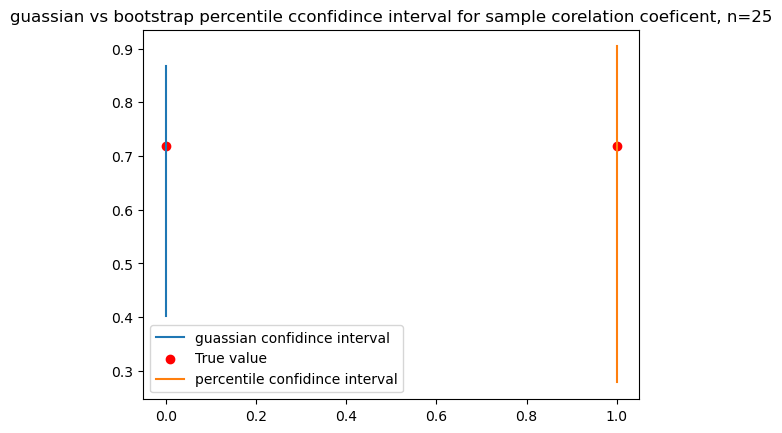
\includegraphics[width=10cm]{homework/homework_5/immages/quistion1b_1.png}
    \item 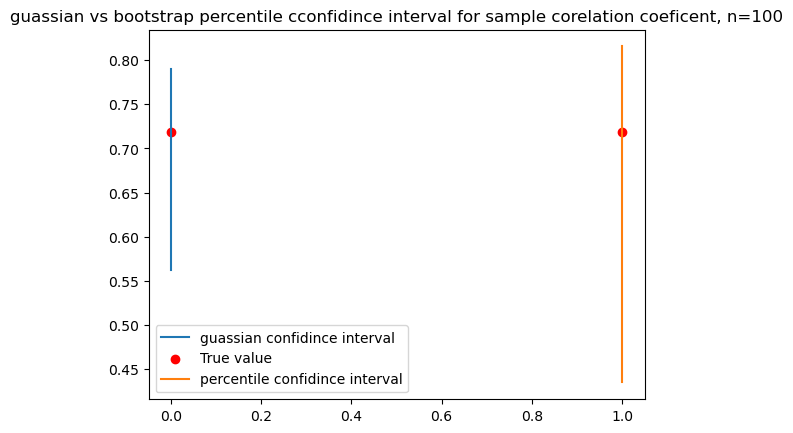
\includegraphics[width=10cm]{homework/homework_5/immages/quistion1b_2.png}
\end{itemize}


\item Estimate and report the probability that the population correlation belongs to each type of confidence interval.
\begin{itemize}
    \color{blue}
    \item using samples of size 25, $\alpha=.05$ and constricting $10,000$ bootstraps i found that the Gaussian confidence intervals captured the population correlation coefficient $90.43\%$ of the time, and the percentile confidence interval $91.81\%$ of the time 
\end{itemize}
\end{enumerate}
\newpage
\item (Confidence intervals for the variance) 
\begin{enumerate}
\item Explain how to build a $1-\alpha$ bootstrap Gaussian confidence intervals for the population variance from $n$ data points.
\begin{itemize}
    \color{blue}
    \item let k be the number of bootstraps you want to make 
    \item initialize a list boostrap\_variances of length k 
    \item loop k times
    \begin{itemize}
    \item sample n individuals randomly, independently and with replacement from your original sample $X$ call this your boot strap sample
    \item calculate the sample variance of your bootstrap sample and add it to the  boostrap\_variances list
        \end{itemize}
    \item calculate the sample variance of the boostrap\_variances list and store it as estimated\_standard\_error 
    \item output a confidence interval as\\ $\mathcal{I}=[se(\text{original sample})-c_{\alpha}*estimated\_standard\_error,se(\text{original sample})+c_{\alpha}*estimated\_standard\_error]$
\end{itemize}

\item Explain how to build a $1-\alpha$ bootstrap percentile confidence intervals for the population variance from $n$ data points.
\begin{itemize}
    \color{blue}
    \item let k be the number of bootstraps you want to make 
    \item initialize a list boostrap\_variances of length k 
    \item loop k times
    \begin{itemize}
    \item sample n individuals randomly, independently and with replacement from your original sample $X$ call this your boot strap sample
    \item calculate the sample variance of your bootstrap sample and add it to the  boostrap\_variances list
        \end{itemize}
    \item calculate a value $q_{\frac{\alpha}{2}}$ such that the proportion of elements in our  boostrap\_variances less than of equal to  $q_{\frac{\alpha}{2}}$ is $\frac{\alpha}{2}$
   \item calculate a value $q_{1-\frac{\alpha}{2}}$ such that the proportion of elements in our  boostrap\_variances less than of equal to  $q_{1-\frac{\alpha}{2}}$ is $1-\frac{\alpha}{2}$
    \item output a confidence interval as\\ $\mathcal{I}=[q_{\frac{\alpha}{2}},q_{1-\frac{\alpha}{2}}]$
\end{itemize}




\item Build 0.95 bootstrap Gaussian and percentile confidence intervals for the population variance of \textit{stature} in \texttt{ANSUR\ II\ MALE\ Public.csv} setting $n=100$. Plot the confidence intervals along with the true population variance. 
\begin{itemize}
    \color{blue}
    \item 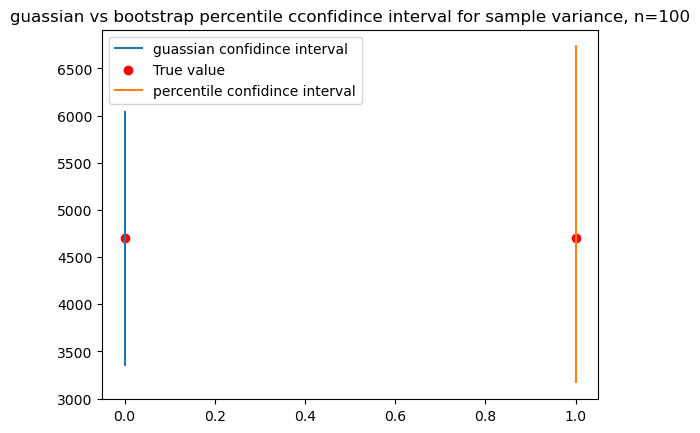
\includegraphics[width=10cm]{homework/homework_5/immages/quistion2b_1.png}
\end{itemize}

\item Estimate and report the probability that the population variance belongs to each type of confidence interval.

\begin{itemize}
    \color{blue}
    \item using samples of size 25, $\alpha=.05$ and constricting $10,000$ bootstraps i found that the Gaussian confidence intervals captured the population correlation coefficient $94.45\%$ of the time, and the percentile confidence interval $93.01\%$ of the time
\end{itemize}

\end{enumerate}

\end{enumerate}
\end{document}
